\documentclass[10pt,a4paper]{article}
\usepackage{tocloft}
\usepackage{commons/course}
\usepackage{booktabs}
\usepackage{graphicx}
\usepackage{tikz}
\usetikzlibrary{arrows.meta,positioning,calc,decorations.pathreplacing,fit}

\definecolor{keywordstyle}{rgb}{0.0, 0.4, 0.8}
\definecolor{stringstyle}{rgb}{0.9, 0.17, 0.31}
\definecolor{commentstyle}{rgb}{0.1, 0.6, 0.2}
\definecolor{numberstyle}{rgb}{0.4, 0.4, 0.4}
\definecolor{backgroundcolor}{rgb}{0.94, 0.97, 1.0}

\lstdefinelanguage{ShellLike}{
	morekeywords={PASS,FAIL,Passed,Failed,Running,Loading,summary,iverilog},
	sensitive=false,
	morecomment=[l]{\#},
	morestring=[b]",
}

\lstset{
	language=ShellLike,
	basicstyle=\ttfamily\scriptsize,
	keywordstyle=\color{keywordstyle}\bfseries,
	stringstyle=\color{stringstyle},
	commentstyle=\color{commentstyle},
	numbers=none,
	keepspaces=true,
	tabsize=2,
	showspaces=false,
	showstringspaces=false,
	showtabs=false,
	breaklines=true,
	breakatwhitespace=false,
	frame=single,
	backgroundcolor=\color{backgroundcolor},
}

\lstdefinestyle{verilog}{
	language=Verilog,
	basicstyle=\ttfamily\scriptsize,
	keywordstyle=\color{keywordstyle}\bfseries,
	commentstyle=\color{commentstyle},
	stringstyle=\color{stringstyle},
	numbers=left,
	numberstyle=\tiny\color{numberstyle},
	frame=single,
	backgroundcolor=\color{backgroundcolor},
	breaklines=true,
	tabsize=2,
}

\newlistof{listofproblems}{lop}{\normalsize فهرست مسائل}
\newcommand{\addproblem}[1]{\addcontentsline{lop}{listofproblems}{\protect\numberline{}#1}}

\begin{document}

\سربرگ{آزمایش ششم}{طراحی یک انکوباتور (\lr{Incubator})}{}{استاد: دکتر انصاری}

\subsubsection*{خلاصه}

در این آزمایش واحد {کنترل دیجیتال} یک سیستم انکوباتور طراحی و پیاده‌سازی شده است. طبق صورت آزمایش، حسگر، \lr{Heater} و \lr{Cooler} خارج از مدار قرار دارند؛ بنابراین دما به‌صورت یک عدد ۸ بیتی وارد مدار می‌شود و عملگرها با سیگنال‌های خروجی نمایش داده می‌شوند که روی برد \lr{FPGA} به \lr{LED} و \lr{Seven Segment} وصل می‌شوند.

واحد کنترل از {دو ماشین حالت} تشکیل شده است که دقیقا از دو نمودار صورت آزمایش گرفته شده‌اند:

\begin{enumerate}
  \item ماشین {اصلی} که تصمیم می‌گیرد \lr{Heater} و \lr{Cooler} روشن باشند یا خاموش (نمودار سمت چپ).
  \item ماشین {سرعت پنکه} که در صورت روشن بودن \lr{Cooler}، دور \lr{Fan} را روی $4$، $6$ یا $8$ دور بر ثانیه تنظیم می‌کند (نمودار سمت راست).
\end{enumerate}

نکته‌ی مهم این است که ماشین دوم {فقط} وقتی فعال است که ماشین اول در حالت $S_2$ باشد؛ چون تنظیم دور پنکه‌ای که خاموش است بی‌معنی است.

\subsubsection*{نمایش دما و نرخ نمونه‌برداری}

صورت آزمایش می‌گوید حسگر دمای بین $-10$ تا $+60$ درجه‌ی سانتیگراد را در قالب یک عدد {۸ بیتی} تحویل می‌دهد و دما {هر یک دقیقه} یک بار خوانده می‌شود.

برای نمایش دما از کد {علامت‌دار مکمل ۲} استفاده شده است، یعنی خود عدد بر حسب درجه:

\begin{center}
\begin{tabular}{@{}lll@{}}
\toprule
{کد ۸ بیتی} & {مقدار} & {توضیح} \\
\midrule
\lr{8'hF6} & $-10$ & سردترین مقدار قابل خواندن \\
\lr{8'h00} & $0$   & صفر درجه \\
\lr{8'h3C} & $+60$ & گرم‌ترین مقدار قابل خواندن \\
\bottomrule
\end{tabular}
\end{center}

مزیت این انتخاب آن است که همه‌ی مقایسه‌ها دقیقا همان‌طور نوشته می‌شوند که در نمودار حالت آمده‌اند؛ یعنی \lr{temp > 35} به جای مقایسه با یک کد میانی که باید جداگانه محاسبه شود.

برای نمونه‌برداری یک‌دقیقه‌ای، ماژول \lr{tick\_gen} یک پالس {تک‌کلاکی} به نام \lr{tick} تولید می‌کند و هر دو ماشین حالت فقط با این پالس یک قدم جلو می‌روند. نسبت تقسیم به‌صورت پارامتر تعریف شده تا در سنتز مقدار واقعی و در شبیه‌سازی یک مقدار کوچک استفاده شود؛ در غیر این صورت تست‌بنچ باید چندین دقیقه زمان واقعی را شبیه‌سازی می‌کرد.

\subsubsection*{معماری کلی}

\begin{center}
\begin{tabular}{@{}l p{8.9cm}@{}}
\toprule
{ماژول} & {مسئولیت} \\
\midrule
\lr{main\_fsm.v}             & ماشین حالت اصلی؛ خروجی‌های \lr{heater} و \lr{cooler} \\
\lr{fan\_fsm.v}              & ماشین حالت سرعت پنکه؛ خروجی \lr{crs} بر حسب \lr{RPS} \\
\lr{tick\_gen.v}             & تولید پالس نمونه‌برداری یک‌دقیقه‌ای \\
\lr{seven\_seg\_decoder.v}   & تبدیل عدد سرعت به کد هفت‌قطعه‌ای \\
\lr{incubator\_controller.v} & اتصال همه‌ی این‌ها به یکدیگر \\
\bottomrule
\end{tabular}
\end{center}

\subsubsection*{ماشین حالت اصلی}

\begin{center}
\begin{latin}
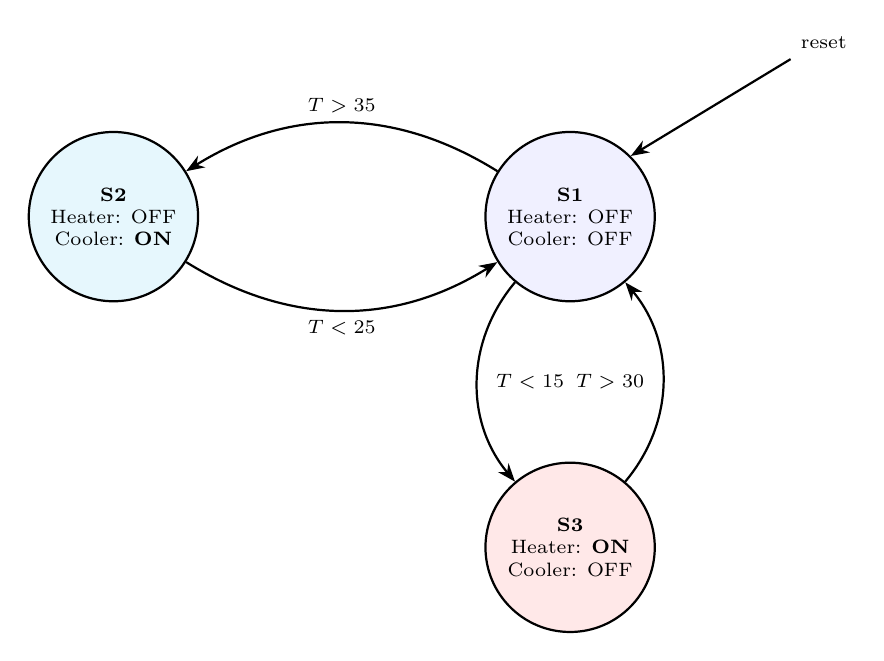
\begin{tikzpicture}[
  st/.style={draw, circle, minimum size=2.15cm, align=center, font=\scriptsize, inner sep=1pt},
  >=Stealth, thick
]
  \node[st, fill=cyan!10]  (s2) at (-5.8,0)  {\textbf{S2}\\Heater: OFF\\Cooler: \textbf{ON}};
  \node[st, fill=blue!6]   (s1) at (0,0)     {\textbf{S1}\\Heater: OFF\\Cooler: OFF};
  \node[st, fill=red!9]    (s3) at (0,-4.2)  {\textbf{S3}\\Heater: \textbf{ON}\\Cooler: OFF};

  \draw[->] (s1) to[bend right=32] node[midway,above,font=\scriptsize]{$T>35$} (s2);
  \draw[->] (s2) to[bend right=32] node[midway,below,font=\scriptsize]{$T<25$} (s1);

  \draw[->] (s1) to[bend right=40] node[midway,right,xshift=3pt,font=\scriptsize]{$T<15$} (s3);
  \draw[->] (s3) to[bend right=40] node[midway,left,xshift=-3pt,font=\scriptsize]{$T>30$} (s1);

  \draw[->] (2.8,2.0) -- (s1.north east)
      node[at start, above right, font=\scriptsize]{reset};
\end{tikzpicture}
\end{latin}
\end{center}

نمودار فقط برای همین چهار گذار برچسب دارد. برای دمایی که هیچ‌کدام از شرط‌های خروجی حالت فعلی را برآورده نکند، ماشین در {همان حالت می‌ماند}. این دقیقا چیزی است که به سیستم خاصیت {پسماند} (\lr{hysteresis}) می‌دهد: یک باند مرده‌ی بین $15$ تا $35$ درجه که جلوی روشن و خاموش شدن پیاپی گرم‌کن و خنک‌کن حول یک نقطه‌ی تنظیم را می‌گیرد.

توجه کنید که همه‌ی مقایسه‌ها {اکید} هستند. مثلا شرط گذار به $S_2$ عبارت است از $T > 35$، بنابراین در دمای دقیقا $35$ درجه خنک‌کن روشن {نمی‌شود}. همین نکته در تست‌بنچ برای هر چهار آستانه جداگانه بررسی شده است.

\begin{latin}
\lstinputlisting[style=verilog]{../rtl/main_fsm.v}
\end{latin}

\subsubsection*{ماشین حالت سرعت پنکه}

\begin{center}
\begin{latin}
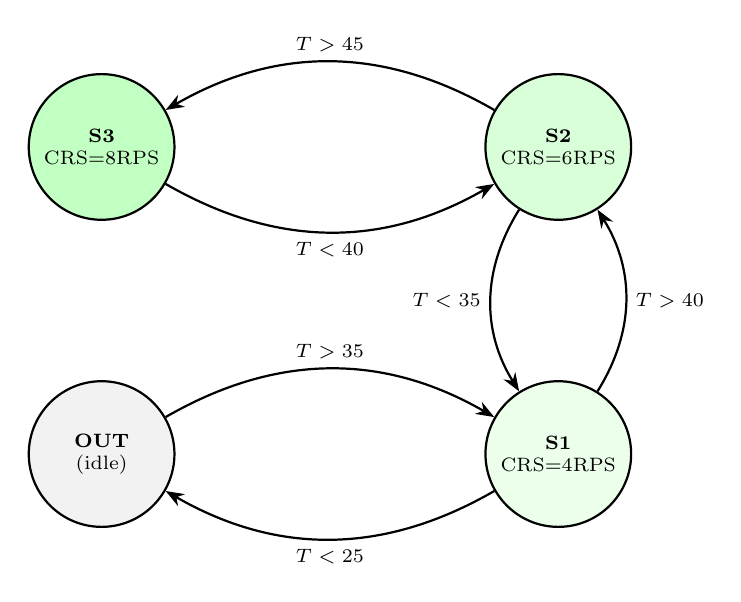
\begin{tikzpicture}[
  st/.style={draw, circle, minimum size=1.85cm, align=center, font=\scriptsize, inner sep=1pt},
  >=Stealth, thick
]
  \node[st, fill=green!24]  (f3)  at (-5.8,3.9)  {\textbf{S3}\\CRS=8RPS};
  \node[st, fill=green!15]  (f2)  at (0,3.9)     {\textbf{S2}\\CRS=6RPS};
  \node[st, fill=green!8]   (f1)  at (0,0)       {\textbf{S1}\\CRS=4RPS};
  \node[st, fill=black!5]   (out) at (-5.8,0)    {\textbf{OUT}\\(idle)};

  \draw[->] (out) to[bend left=30]  node[midway,above,font=\scriptsize]{$T>35$} (f1);
  \draw[->] (f1)  to[bend left=30]  node[midway,below,font=\scriptsize]{$T<25$} (out);

  \draw[->] (f1) to[bend right=32] node[midway,right,font=\scriptsize]{$T>40$} (f2);
  \draw[->] (f2) to[bend right=32] node[midway,left,font=\scriptsize]{$T<35$} (f1);

  \draw[->] (f2) to[bend right=30] node[midway,above,font=\scriptsize]{$T>45$} (f3);
  \draw[->] (f3) to[bend right=30] node[midway,below,font=\scriptsize]{$T<40$} (f2);
\end{tikzpicture}
\end{latin}
\end{center}

طبق متن صورت آزمایش، این ماشین تنها زمانی فعال است که ماشین اصلی در حالت $S_2$ باشد و در غیر این صورت {وارد حالت \lr{OUT} خود می‌شود}. بنابراین سیگنال \lr{enable} که پایین می‌آید، حالت را {مجبور} به \lr{OUT} می‌کند، نه اینکه صرفا آن را منجمد نگه دارد. نتیجه این است که هر بار ورود دوباره به $S_2$، پنکه از پایین‌ترین پله‌ی نردبان سرعت شروع می‌کند، نه از سرعتی که قبلا داشته است.

\begin{latin}
\lstinputlisting[style=verilog]{../rtl/fan_fsm.v}
\end{latin}

\subsubsection*{نکته‌ی طراحی: هم‌زمانی دو ماشین حالت}

مهم‌ترین نکته‌ی ظریف این آزمایش، {لحظه‌ی دقیق} فعال یا غیرفعال شدن ماشین دوم است.

اگر سیگنال \lr{enable} را مستقیما به خروجی \lr{cooler} (یعنی {حالت فعلی} ماشین اصلی) وصل کنیم، در همان \lr{tick} که ماشین اصلی از $S_2$ خارج می‌شود، مقدار \lr{cooler} هنوز مقدار قدیمی است. در نتیجه ماشین پنکه یک قدم {اضافه} برمی‌دارد و برای یک دوره‌ی کامل نمونه‌برداری (یعنی یک دقیقه‌ی واقعی) وضعیتی نمایش داده می‌شود که در آن خنک‌کن خاموش است ولی پنکه هنوز در حال چرخش است. این دقیقا همان چیزی است که متن آزمایش می‌گوید بی‌معنی است.

راه‌حل این است که ماشین پنکه با {حالت بعدی} ماشین اصلی گیت شود:

\begin{latin}
\begin{lstlisting}[style=verilog,numbers=none]
// in main_fsm: the state this FSM will hold AFTER the current tick
assign cooler_next = (nxt == S2);

// in incubator_controller: gate the fan on the next state, not the current one
fan_fsm u_fan ( ... .enable(cooler_next), ... );
\end{lstlisting}
\end{latin}

با این تغییر، همان \lr{tick} که خنک‌کن را خاموش می‌کند، پنکه را هم در \lr{OUT} پارک می‌کند و هر دو ماشین بر اساس یک نمونه‌ی دما به‌صورت سازگار عمل می‌کنند. در سمت ورود هم رفتار درست است: چون شرط $T>35$ هم باعث ورود ماشین اصلی به $S_2$ می‌شود و هم شرط گذار \lr{OUT} به $S_1$ در ماشین پنکه است، خنک‌کن در همان لحظه‌ی روشن‌شدن سرعت اولیه‌ی $4$ \lr{RPS} خود را می‌گیرد.

\subsubsection*{اتصال ماژول‌ها و خروجی‌های برد}

طبق تأکید صورت آزمایش، به جای \lr{Heater} و \lr{Cooler} واقعی، خروجی‌ها با \lr{LED} و \lr{Seven Segment} نمایش داده می‌شوند. بنابراین خروجی \lr{crs} علاوه بر مقدار عددی، به‌صورت کد هفت‌قطعه‌ای (\lr{crs\_seg}) هم بیرون داده می‌شود تا طراحی بدون منطق واسط اضافه روی برد قابل استفاده باشد.

\begin{center}
\begin{tabular}{@{}lll p{6.1cm}@{}}
\toprule
{سیگنال} & {جهت} & {پهنا} & {توضیح} \\
\midrule
\lr{Clk}        & ورودی & ۱ & کلاک برد \\
\lr{RstN}       & ورودی & ۱ & ریست ناهم‌گام فعال‌پایین \\
\lr{temp}       & ورودی & ۸ & دمای حسگر، علامت‌دار، $-10$ تا $+60$ \\
\lr{heater}     & خروجی & ۱ & \lr{LED} گرم‌کن \\
\lr{cooler}     & خروجی & ۱ & \lr{LED} خنک‌کن \\
\lr{crs}        & خروجی & ۴ & دور پنکه بر حسب \lr{RPS} ($0/4/6/8$) \\
\lr{crs\_seg}   & خروجی & ۷ & همان مقدار، کدشده برای \lr{Seven Segment} \\
\bottomrule
\end{tabular}
\end{center}

\begin{latin}
\lstinputlisting[style=verilog]{../rtl/incubator_controller.v}
\end{latin}

\subsubsection*{شکل موج}

شکل‌موج یک چرخه‌ی کامل حرارتی را نشان می‌دهد: از باند مرده شروع می‌شود، به سرما می‌رود و گرم‌کن روشن می‌شود، دوباره گرم می‌شود تا خنک‌کن روشن شود و پنکه نردبان $4 \to 6 \to 8$ را بالا و پایین برود، و در پایان همه‌چیز خاموش می‌شود.

\begin{center}
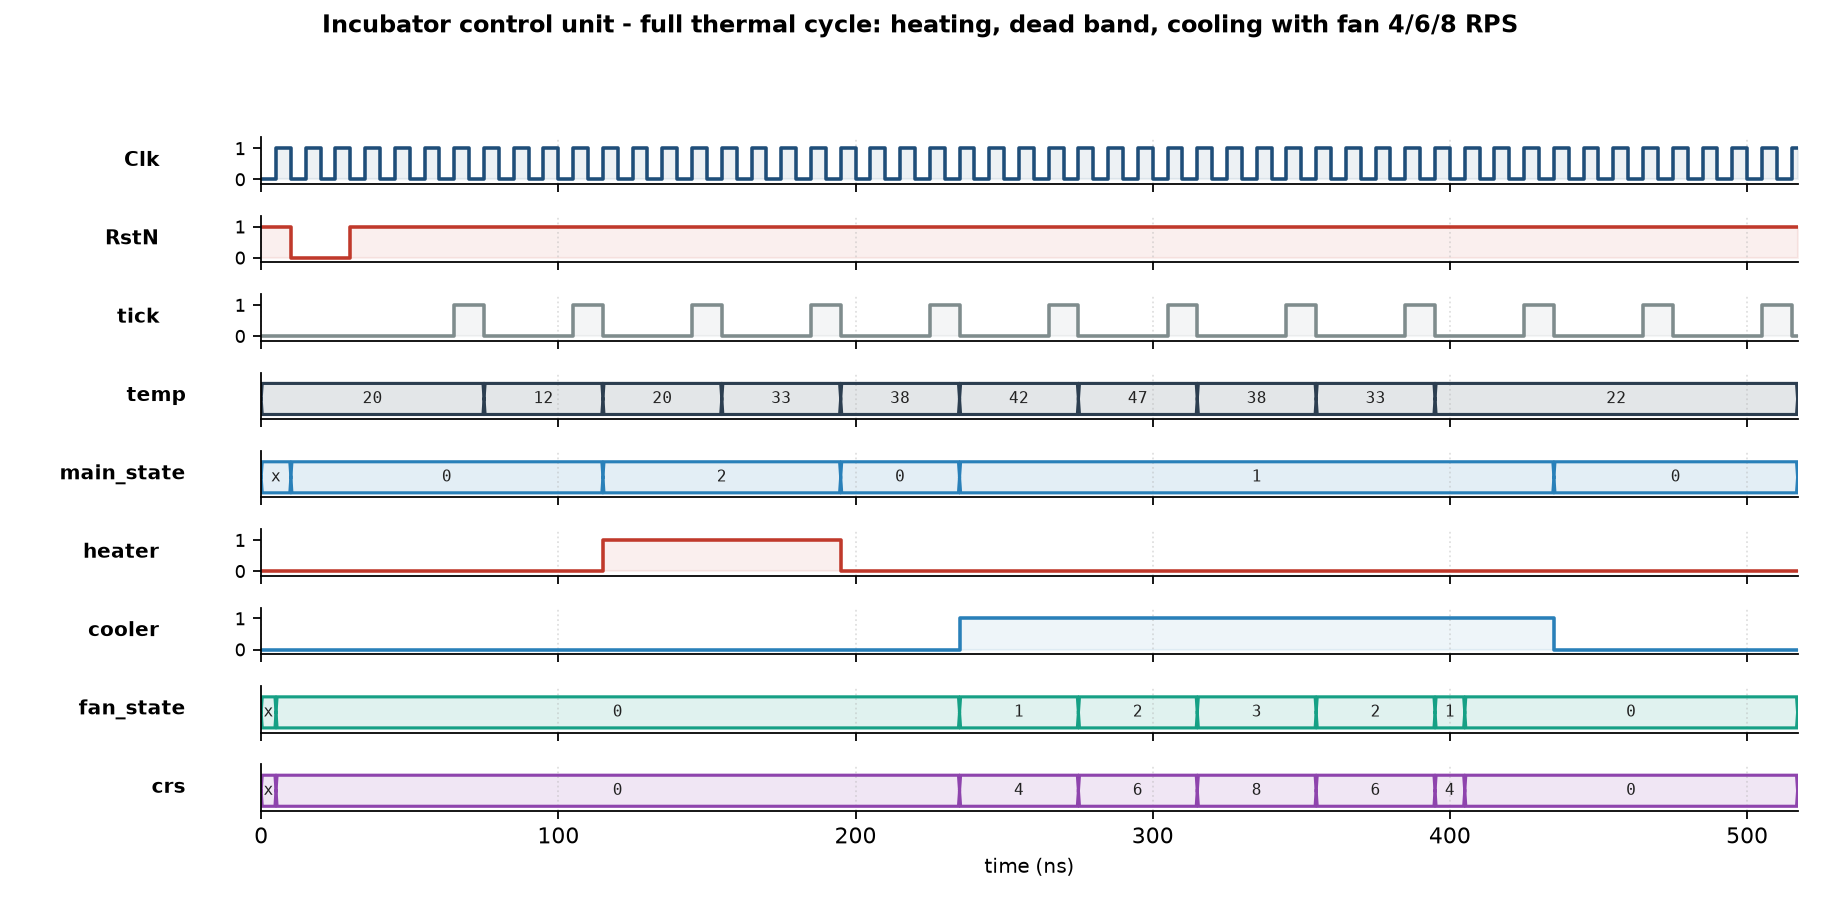
\includegraphics[width=\textwidth]{figs/wave_incubator.png}\\[0.4em]
\end{center}

نکات قابل مشاهده: در دمای $12$ درجه گرم‌کن روشن می‌شود و در $20$ درجه {همچنان روشن می‌ماند} — این همان خاصیت پسماند است، نه اشکال. در $33$ درجه گرم‌کن خاموش می‌شود و در $38$ درجه خنک‌کن روشن شده و پنکه بلافاصله روی $4$ \lr{RPS} قرار می‌گیرد. سپس با $42$ و $47$ درجه به $6$ و $8$ می‌رسد و در مسیر برگشت دوباره پایین می‌آید. در پایان با رسیدن دما به $22$ درجه، \lr{cooler} پایین می‌آید و {در همان لحظه} مقدار \lr{crs} صفر می‌شود؛ یعنی همان رفتاری که در بخش قبل درباره‌اش صحبت شد.

\subsubsection*{تست‌بنچ اول: مقایسه با مدل مرجع}

تست‌بنچ اصلی یک {مدل مرجع} مستقل از هر دو نمودار حالت نگه می‌دارد و بعد از هر نمونه‌برداری، حالت هر دو ماشین به‌همراه خروجی‌های \lr{heater}، \lr{cooler} و \lr{crs} را با آن مقایسه می‌کند.

پوشش تست شامل این موارد است: ریست، باند مرده‌ی $15$ تا $35$ درجه، چرخه‌ی گرمایش، چرخه‌ی سرمایش با کل نردبان پنکه، ریست وسط کار، و مهم‌تر از همه یک {جاروب کامل}: از چهار پیکربندی مختلف $(\text{main}, \text{fan})$ شروع می‌شود و از هر کدام تمام دماهای بازه‌ی $-10$ تا $+60$ اعمال و با مدل مقایسه می‌شود.

علاوه بر این، یک \lr{invariant} به‌صورت پیوسته بررسی می‌شود:

\begin{latin}
\begin{lstlisting}[style=verilog,numbers=none]
always @(posedge Clk)
    if (RstN && !cooler && crs !== 4'd0) ... // FAIL
\end{lstlisting}
\end{latin}

این بررسی در {هر} لبه‌ی کلاک انجام می‌شود، نه فقط در نقاط نمونه‌برداری؛ بنابراین حتی یک لحظه چرخش پنکه در زمان خاموشی خنک‌کن هم تست را رد می‌کند.

\begin{latin}
\lstinputlisting[style=verilog]{../tb/tb_incubator.v}
\end{latin}

\subsubsection*{تست‌بنچ دوم: انطباق با نمودار}

مدل مرجع بررسی قدرتمندی است، اما یک ضعف ذاتی دارد: مدلی که به دست {همان} طراح نوشته شده، ممکن است همان برداشت اشتباه از صورت مسئله را تکرار کند. دقیقا همین اتفاق در این آزمایش افتاد — هم \lr{RTL} و هم مدل مرجع، در ابتدا اجازه می‌دادند پنکه در لحظه‌ی خاموش شدن خنک‌کن یک قدم اضافه بردارد و هر دو با هم موافق بودند، پس تست سبز بود.

به همین دلیل یک تست‌بنچ دوم نوشته شد که مستقیما از {روی نمودارهای صورت آزمایش} و بدون هیچ مدل مشترکی، فهرستی از رفتارهایی را که باید برقرار باشند بررسی می‌کند: مقایسه‌های اکید روی هر شش آستانه، پله‌های $4/6/8$، صفر بودن سرعت در تمام حالت‌هایی که خنک‌کن خاموش است، و شروع دوباره از پایین نردبان پس از بازگشت به $S_2$. همین تست بود که اشکال را پیدا کرد.

\begin{latin}
\lstinputlisting[style=verilog]{../tb/tb_incubator_spec.v}
\end{latin}

\subsubsection*{نتایج تست}

\begin{latin}
\lstinputlisting[basicstyle=\ttfamily\scriptsize]{figs/test_run_output.txt}
\end{latin}

\subsubsection*{جمع‌بندی}

در این آزمایش دو ماشین حالت طراحی شد که یکی از آن‌ها {مشروط} به وضعیت دیگری فعال می‌شود. تجربه‌ی اصلی این بود که وقتی دو ماشین حالت روی یک رویداد مشترک (اینجا پالس نمونه‌برداری) کار می‌کنند، باید دقیقا مشخص کرد که هر کدام بر اساس {کدام نسخه} از حالت دیگری تصمیم می‌گیرد؛ حالت فعلی یا حالت بعدی. انتخاب اشتباه، مداری می‌سازد که نه در شبیه‌سازی خطای نحوی می‌دهد و نه لزوما در تست‌های ساده دیده می‌شود، ولی رفتار فیزیکی نادرستی تولید می‌کند.

در نهایت، خاصیت پسماند در این طراحی یک ویژگی عمدی است نه اتفاقی. باند مرده‌ی $15$ تا $35$ درجه باعث می‌شود سیستم حول یک نقطه‌ی تنظیم دچار روشن و خاموش شدن پیاپی نشود، که هم برای عمر عملگرها و هم برای پایداری دمای داخل محفظه مطلوب است.

\pagebreak
\subsubsection*{خروجی سنتز (\lr{Quartus Prime})}

طرح روی \lr{Intel Quartus Prime Lite Edition 21.1.0} با موجودیت سطح‌بالای \lr{incubator\_controller} (شامل \lr{main\_fsm}، \lr{fan\_fsm}، \lr{tick\_gen} و \lr{seven\_seg\_decoder}) سنتز و Place \& Route شد. دستگاه هدف: \lr{Cyclone V} (\lr{5CGXFC7C7F23C8}).

\begin{center}
\begin{tabular}{@{}lr@{}}
\toprule
{مورد} & {نتیجه} \\
\midrule
وضعیت کامپایل & موفق ($0$ خطا، $17$ هشدار) \\
\lr{Logic utilization (ALMs)} & $44 / 56480$ ($<1\%$) \\
\lr{Total registers} & $41$ \\
\lr{Total pins} & $28 / 268$ ($10\%$) \\
\lr{Block memory bits} & $0$ \\
\lr{DSP Blocks} & $0$ \\
\bottomrule
\end{tabular}
\end{center}

\begin{center}

\includegraphics[width=\textwidth]{figs/quartus_synthesis.jpg}
\end{center}

\end{document}
